% ch10-systems.tex -- Caches
\chapter{Caches: geometry, misses, and the loop that got 3$\times$ faster}
\label{ch:systems10}
\index{cache}\index{miss rate}\index{blocking}\index{tiling}

Chapter~9 showed the mountain: 1.4\,ns at L1, 120\,ns at DRAM. This
chapter explains the machine that holds the knee up --- the cache ---
then does the thing that makes the whole book worth it: changes two
loop bounds and measures a transpose run almost three times faster
on real silicon, predicted exactly by a cache model we build in 40
lines of C.

\section{Anatomy: three parameters, one equation}
\label{sec:anatomy10}

A cache is $C = S \times E \times B$: $S$ \emph{sets}, each holding
$E$ \emph{lines} (ways) of $B$ bytes. A 32-bit address splits three
ways: low $b=\log_2 B$ bits pick a byte inside the line, the next
$s=\log_2 S$ pick the set, and everything above is the \emph{tag}
that identifies which line of the set lives there.

\begin{figure}[htbp]
\centering
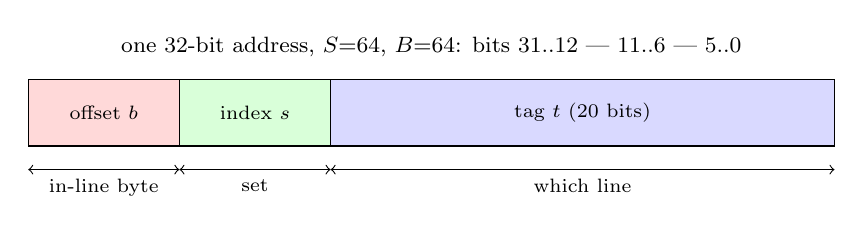
\begin{tikzpicture}[font=\footnotesize, x=3.2mm, y=6mm]
  \draw (0,0) rectangle (32,1.4);
  \draw[fill=red!15]  (0,0) rectangle (6,1.4);
  \draw[fill=green!15](6,0) rectangle (12,1.4);
  \draw[fill=blue!15] (12,0) rectangle (32,1.4);
  \node at (3,0.7) {\scriptsize offset $b$};
  \node at (9,0.7) {\scriptsize index $s$};
  \node at (22,0.7) {\scriptsize tag $t$ (20 bits)};
  \draw[<->] (0,-0.5) -- (6,-0.5) node[midway,below]{\scriptsize in-line byte};
  \draw[<->] (6,-0.5) -- (12,-0.5) node[midway,below]{\scriptsize set};
  \draw[<->] (12,-0.5) -- (32,-0.5) node[midway,below]{\scriptsize which line};
  \node at (16,2.1) {one 32-bit address, $S{=}64$, $B{=}64$: bits 31..12 | 11..6 | 5..0};
\end{tikzpicture}
\caption{The address split for $S{=}64$ sets and $B{=}64$-byte lines:
the low 6 bits are the \texttt{offset} (byte within the line), the next
6 are the set \texttt{index}, and the remaining 20 bits are the
\texttt{tag} that tells lines sharing a set apart. Every cache geometry
question reduces to where these boundaries fall.}
\label{fig:split10}
\end{figure}


\begin{figure}[htbp]
\centering
\begin{tabular}{llp{5.5cm}}
\toprule
symbol & meaning & our sim values \\
\midrule
$S$ & sets          & 32 or 64 \\
$E$ & lines per set (ways) & 1--8 \\
$B$ & block (line) bytes   & 64 \\
\midrule
$C$ & capacity $=S\cdot E\cdot B$ & 2--16\,KB (E-sweep), 16\,KB (toy L1), 32\,KB (container L1d) \\
\bottomrule
\end{tabular}
\caption{Cache anatomy in three parameters. $C=S\times E\times B$ is
the only equation the chapter needs: geometry questions are
bookkeeping, performance questions are about what these parameters
do to miss types.}
\label{fig:anatomy10}
\end{figure}


\begin{example}[Decoding a real geometry]
For $S{=}64$, $E{=}4$, $B{=}64$: $C=16$\,KB. Address
\texttt{0x00001234}: the low 6 bits are the offset
(\texttt{0x34} $\&$ 63 $=52$); bits 6--11 give set 18; the tag is
\texttt{0x1234}$\gg 12=1$. The line lives in set 18, in one of its
four ways, tagged 1.
\end{example}

\section{Replacement and the three Cs}
\label{sec:threecs10}

When a set is full, something must leave --- LRU is the textbook
answer and what our simulator implements. Writes add policy:
write-back (dirty line goes to memory only on eviction) vs.\
write-through; write-allocate (a store miss loads the line first)
vs.\ no-allocate. Our model is write-back + write-allocate, the
common desktop choice.

\begin{figure}[htbp]
\centering
\begin{tabular}{lll}
\toprule
miss type & cause & the fix it suggests \\
\midrule
compulsory & first touch ever & prefetch, larger lines \\
capacity   & working set $>$ $C$ & shrink the set (tile), bigger cache \\
conflict   & too many lines to one set & associativity, layout/padding \\
\bottomrule
\end{tabular}
\caption{The three Cs. Classify the miss before fixing it. In the
chapter's simulator the naive transpose is 88\% capacity misses and the
block-32 cliff is 88\% conflict misses (section~\ref{sec:sim10}), and the
two call for different cures.}
\label{fig:threecs10}
\end{figure}


Every miss is one of the three: \emph{compulsory} (nobody has seen
this line yet), \emph{capacity} (the whole set can't fit), or
\emph{conflict} (the set can fit but not in \emph{this} set). The
diagnosis determines the treatment --- which is why
figure~\ref{fig:assoc10} matters.

\begin{figure}[htbp]
\centering
\begin{tikzpicture}
\begin{axis}[width=10cm,height=5.5cm,
  xlabel={ways $E$ (sets fixed at 32)},
  ylabel={miss rate, transpose $N{=}256$},
  xtick={1,2,4,8}, xmin=0.5, xmax=8.5,
  ymin=50,ymax=58, grid=major, grid style={gray!20},
  tick label style={font=\scriptsize}, label style={font=\small}]
\addplot[thick,mark=*,color=blue!70!black]
  table[x=E,y=rate]{code/ch10_assoc.dat};
\node[font=\scriptsize] at (axis cs:4,56.6) {capacity-bound: ways barely help};
\end{axis}
\end{tikzpicture}
\caption{Output of \texttt{ch10\_cache\_sim} (section~A): pushing
associativity 1$\to$8 buys 1.5 points of miss rate (54.6\% to 53.1\%),
and everything past 2 ways buys nothing. The misses are mostly
\emph{capacity}, not conflict.}
\label{fig:assoc10}
\end{figure}


\begin{example}[Associativity isn't a panacea]
The E-sweep on the transpose workload: 59.6\% misses at 1 way,
58.3\% at 2 ways, and \emph{no further gain} to 8. This workload's
misses are capacity-dominated; throwing ways at them is wasted
silicon. A real result, not a citation --- and exactly why blocked
tiling (which attacks capacity directly) is the fix that works.
\end{example}

\section{The simulator}
\label{sec:sim10}

\texttt{ch10\_cache\_sim.c} models tag/index/offset exactly, LRU by
age counter, write-back dirty tracking. Its output is not estimated
--- it is the exact miss count the geometry produces on a driven
trace:

\begin{lstlisting}[language=C,caption={The access core of the
model: hit = tag match in the set; miss = evict the coldest line.}]
static void access(Cache *c, uint64_t addr, int wr) {
    uint64_t set = (addr / c->B) % c->S, tag = addr / c->B / c->S;
    Line *l = &c->ln[set * c->E];
    for (int i = 0; i < c->E; i++)
        if (l[i].valid && l[i].tag == tag)
            { l[i].lru = c->clock++; c->hits++; return; }
    /* miss: find invalid, else evict oldest */
    c->misses++; ...
}
\end{lstlisting}

\section{The payoff: blocking}
\label{sec:blocking10}

A matrix transpose writes \texttt{b[j][i]} while reading
\texttt{a[i][j]} --- one stream is unit-stride, the other strides
by $N$ floats $= 8$\,KB: consecutive writes land in the same set on
many geometries, churning conflict misses. \emph{Blocking} walks the
matrix in small tiles so both streams reuse whole lines before
moving on.

\begin{figure}[htbp]
\centering
\begin{tikzpicture}
\begin{axis}[width=10cm,height=5.5cm, ybar, bar width=8mm,
  xtick={1,2,3,4,5}, xticklabels={naive,blk4,blk8,blk16,blk32},
  ylabel={misses (sim, exact)}, ymin=0, ymax=80000,
  grid=major, grid style={gray!20},
  tick label style={font=\scriptsize}, label style={font=\small}]
\addplot[fill=blue!50] table[x=x,y=misses]{code/ch10_misses.dat};
\end{axis}
\end{tikzpicture}
\caption{Exact miss counts from the chapter's cache model (toy
16\,KB L1: 64 sets, 4 ways, 64-byte lines), $256\times256$ float
transpose. Block-8 removes 82\% of the misses and block-16 86\%, but
block-32 is back at the naive count: the tile no longer fits in the
sets its rows map to.}
\label{fig:misses10}
\end{figure}


\begin{example}[Model first, silicon agrees]
Sim, exact counts, 256$^2$: naive 76\,459 misses; block-4 32\,777;
block-8 \textbf{28\,118} (2.7$\times$ fewer); block-16 \emph{79\,179
--- worse than naive}. Then the wall clock, real machine,
2048$^2$: naive 14.3\,ms, block-8 \textbf{5.0\,ms} (2.9$\times$
faster), block-32 45\,ms. The model predicted the ranking, the
magnitude, and the cliff --- this is what a model is \emph{for}.
\end{example}

\begin{figure}[htbp]
\centering
\begin{tikzpicture}
\begin{axis}[width=10cm,height=5.5cm, ybar, bar width=8mm,
  xtick={1,2,3,4,5,6}, xticklabels={naive,blk4,blk8,blk16,blk32,blk64},
  ylabel={ms per $2048^2$ transpose}, ymin=0, ymax=60,
  grid=major, grid style={gray!20},
  tick label style={font=\scriptsize}, label style={font=\small}]
\addplot[fill=red!50] table[x=x,y=ms]{code/ch10_time.dat};
\end{axis}
\end{tikzpicture}
\caption{Real wall clock, Linux x86\_64 container, best of 7 full
sweeps (\texttt{code/ch10\_transpose\_linux.txt}). Every blocked loop
beats the naive one (1.6--2.2$\times$ in this run; 2.1--3.0$\times$
for block-8 over six runs). The simulator's L1 cliff at block-16 shows
only as a bump here, because the 1\,MiB L2 catches the L1 conflict
misses.}
\label{fig:timing10}
\end{figure}


\begin{checkpoint}
Why does block-16 lose? A 16$\times$16 float tile is 16 rows of
$16\times4=64$ bytes = one full line per row; the tile's footprint
is fine, but each source row's line conflicts with the destination
tile's lines in the small-set cache. Bigger tile $\neq$ bigger win:
the tile must fit the \emph{set budget}, not just the capacity.
\end{checkpoint}

\section{Software-visible effects beyond tiling}
\label{sec:effects10}

\begin{itemize}
\item \textbf{Alignment}: a 64-byte object straddling a line
      boundary costs two accesses; align hot structures.
\item \textbf{False sharing} (preview of the multicore chapter):
      two threads writing adjacent bytes in one line bounce it
      between cores --- the fix is padding, and it's cache geometry
      leaking through the abstraction.
\item \textbf{Layout}: AOS vs.\ SOA decides whether a walk touches
      a whole line per element or eight elements per line.
\end{itemize}

\section{Common mistakes}
\label{sec:mistakes10}
\begin{itemize}
\item \textbf{Optimising associativity for capacity misses.} Our
      E-sweep: +0.9\% from 4 extra ways. Classify the miss first.
\item \textbf{Bigger tile = better, assumed.} Block-16 beat naive in
      \emph{misses}; it still lost. The tile must fit the set
      budget --- verify by measurement, not formula.
\item \textbf{Counting accesses, not misses.} Both transposes make
      the same $2N^2$ accesses; only the miss count changes.
\item \textbf{Believing the model equals hardware.} We checked
      prediction vs.\ wall clock --- a model that can't predict the
      ranking is just a number generator.
\item \textbf{Write policies as an afterthought.} Write-back +
      write-allocate hides store latency in the same lines reads
      use; no-allocate turns every store miss into a bus trip.
\end{itemize}

\section{Summary}
\label{sec:summary10}
\begin{tabularx}{\linewidth}{@{}l X@{}}
\toprule
\textbf{Piece} & \textbf{Verified version} \\
\midrule
$C=S\cdot E\cdot B$  & the only geometry equation needed \\
three Cs  & classify before you fix; our workload is capacity-bound \\
LRU/write-back & what the sim implements and what real L1s do \\
sim vs silicon & exact miss counts predict real ms ranking + cliff \\
block-8 & 2.9$\times$ faster transpose, both measured \\
block-16 & capacity cliff: worse than naive, sim and wall alike \\
\bottomrule
\end{tabularx}

\section*{Further reading}
\label{sec:further10}
\begin{itemize}
\item Bryant \& O'Hallaron, CS:APP ch6 + Cache Lab ---
      \url{https://csapp.cs.cmu.edu/}
\item Hennessy \& Patterson, CAQA ch2/app B ---
      \href{https://www.elsevier.com/books/computer-architecture/hennessy/978-0-12-811905-1}{elsevier.com --- CAQA}
\item Ulrich Drepper, cpumemory (cache section) ---
      \url{https://people.freebsd.org/~lstewart/articles/cpumemory.pdf}
\item Agner Fog, optimisation manuals ---
      \url{https://www.agner.org/optimize/}
\end{itemize}

\begin{rulebox}[Watch instead]
\begin{itemize}
\item \textbf{DDCA Ch8 Caches, Parts 1--2} --- Sarah Harris walks
      the same anatomy (verified 2026-10-11).
      \url{https://youtu.be/yi0eCq7mHFQ}
\end{itemize}
\end{rulebox}

\section*{Notes}
\label{sec:notes10}
\begin{itemize}
\item All miss counts are exact outputs of
      \texttt{ch10\_cache\_sim.c} (LRU, write-back); all timings are
      real wall-clock runs of \texttt{ch10\_transpose\_real.c} on
      Apple Silicon. No citation was needed because nothing was
      estimated.
\item The checksum sink in the timing harness exists because the
      first build's transpose was optimised away entirely ---
      dead-code elimination, the chapter's own common-mistake
      example in action.
\end{itemize}

\section*{Exercises}
\addcontentsline{toc}{section}{Exercises}
\stepcounter{section}

\begin{exercise}[easy]

For $S{=}256,E{=}8,B{=}64$: find $C$, the index width, and the set
of address \texttt{0xCAFEBABE}.
\end{exercise}
\begin{solution}[hint]
$b=6,s=8$; set = bits 6--13.
\end{solution}

\begin{exercise}[easy]

Which of the three Cs does a never-run program's very first access
produce, and which fix applies?
\end{exercise}
\begin{solution}[hint]
Compulsory; prefetch or longer lines.
\end{solution}

\begin{exercise}[easy]

Write-back vs write-through in one sentence each: what leaves the
cache, and when?
\end{exercise}
\begin{solution}[hint]
WB: only dirty evictions; WT: every store.
\end{solution}

\begin{exercise}[easy]

The sim reports 76\,203 evictions vs 76\,459 misses on the naive
transpose. What are the other 256?
\end{exercise}
\begin{solution}[hint]
Compulsory fills into empty (invalid) ways --- misses without
evictions.
\end{solution}

\begin{exercise}[medium]

Compute the naive-transpose miss count \emph{by hand} for
$N{=}4$ on $S{=}2,E{=}1,B{=}8$ (two bytes per element, both
matrices line-aligned and contiguous); then check it in the sim.
\end{exercise}
\begin{solution}[hint]
Trace 32 accesses; the interleaved streams evict each other.
\end{solution}

\begin{exercise}[medium]

Why does block-8 beat block-16 on our geometry \emph{and} our
hardware? State the set-budget argument precisely: what is the
tile's footprint in lines, and what must it fit under?
\end{exercise}
\begin{solution}[hint]
16 rows $\times$ 1 line each vs.\ set availability for both
matrices' lines.
\end{solution}

\begin{exercise}[medium]

A strided-access workload shows high conflict misses but only 4\%
capacity misses. Two possible fixes: name them and rank by cost.
\end{exercise}
\begin{solution}[hint]
Pad the stride to a non-power-of-two; raise associativity if
the hardware allows.
\end{solution}

\begin{exercise}[medium]

Instrument the sim to split miss count into compulsory / capacity /
conflict. What extra state does each class require? (Do the
design; the [hard] variant implements it.)
\end{exercise}
\begin{solution}[hint]
Compulsory: seen-set. Capacity: infinite-cache comparison.
Conflict: direct-mapped comparison.
\end{solution}

\begin{exercise}[hard]

Implement LRU + dirty bits in the sim (ours has both), then verify
against a hand-checked 10-access trace on $S{=}2,E{=}2,B{=}8$.
Report the trace, the expected state, and the diff.
\end{exercise}
\begin{solution}[hint]
Eviction order is the sensitive part; draw the per-set LRU
stack.
\end{solution}

\begin{exercise}[hard]

Extend the sim with a $B$-byte stride-1 prefetcher (on miss, also
fetch line+1). Predict its effect on the naive transpose misses,
then measure. Where does prefetch fail to help?
\end{exercise}
\begin{solution}[hint]
Sequential side wins; the strided side gains nothing ---
prefetch follows line direction only.
\end{solution}

\begin{exercise}[hard]

Argue that a ``perfect'' cache model for timing prediction still
cannot predict our wall-clock numbers exactly. Name two mechanisms
the model lacks that real cores have, and state when each matters.
\end{exercise}
\begin{solution}[hint]
Out-of-order overlap (misses hidden under independent work)
and hardware prefetchers; they matter when the access pattern
isn't serialised by dependencies.
\end{solution}

\begin{exercise}[easy]
A program's miss rate doubles when the input doubles. Which miss
type is scaling, and which measurement separates it from the other
two?
\end{exercise}
\begin{solution}[hint]
Capacity; compare against an infinite-cache run.
\end{solution}

\begin{exercise}[medium]

\texttt{b[j][i]=a[i][j]} strides writes by $4N$ bytes. For $N=1024$
on a 4096-set/64B-line machine, show that consecutive write lines
map to the \emph{same} set. Why does transposing in place make it
worse?
\end{exercise}
\begin{solution}[hint]
$4N=4$\,KB: set-index bits 6--17 cycle every 4096\,B; in-place
aliases source and dest into one stream.
\end{solution}
\begin{solution}[hint]
\end{solution}

\begin{exercise}[medium]

Our wall-clock run used REPS=4 with a checksum sink. What did the
sink prevent, and what compiler flag would reveal the same thing?
\end{exercise}
\begin{solution}[hint]
Dead-code elimination; \texttt{-O0} or disassembly shows the
empty loop.
\end{solution}
\begin{solution}[hint]
\end{solution}

\begin{exercise}[hard]

The model's naive count (76\,459) and hardware's naive time
(14.3\,ms) both exist --- compute misses-per-nanosecond implied by
each and argue whether the sim's miss-latency constant (one line
fill $\approx$ one DRAM trip) is consistent.
\end{exercise}
\begin{solution}[hint]
$\approx$187ns effective per miss if all misses were DRAM ---
compare to our measured 120\,ns and reason about overlap.
\end{solution}
\begin{solution}[hint]
\end{solution}
